%!TEX root = ./template-skripsi.tex
%-------------------------------------------------------------------------------
%                            BAB III
%               		PEMBAHASAN
%-------------------------------------------------------------------------------

\chapter{HASIL DAN PEMBAHASAN}

Dalam penelitian ini tahapan yang akan dilakukan adalah seperti gambar di bawah ini

\begin{figure}[H]
	\centering
	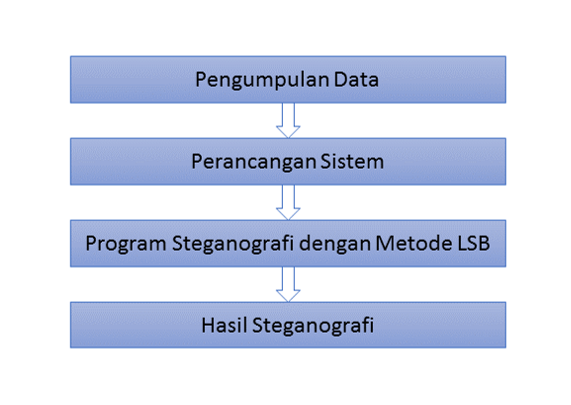
\includegraphics[width=0.8\textwidth]{gambar/alur_penelitian}
	\caption{Alur Penelitian}
	\label{alur_penelitian}
\end{figure}

\section{Pengumpulan Data}
\begin{enumerate}
	\item Studi Pustaka\\
	Penulis mendapatkan informasi yang berkaitan dengan steganografi melalui buku referensi dan juga dalam bentuk \emph{e-book}. Penulis juga mencari informasi melalui berbagai situs di internet yang sesuai dengan topik.	
	\item Studi Literatur\\
	Penulis mencoba mencari perbandingan dengan studi sejenis dari beberapa karya ilmiah lokal maupun internasional, seperti jurnal dan skripsi.	 
\end{enumerate}

\section{Perancangan Sistem}

	\subsection{Proses Penyisipan (\emph{Encoding}) pesan ke Citra \emph{Digital}}
	
	\begin{figure}[H]
		\centering
		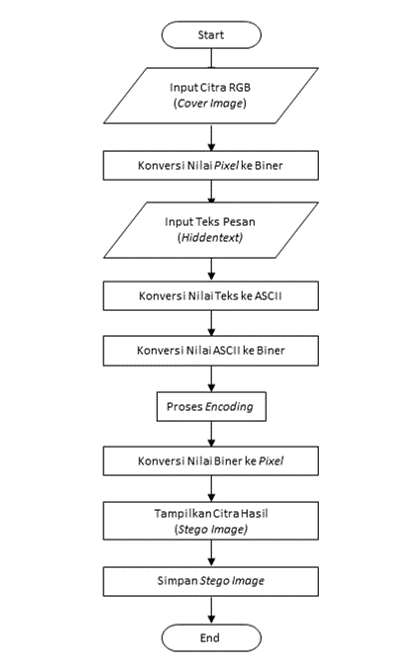
\includegraphics[height=0.8\textheight]{gambar/penyisipan3}
		\caption{\emph{Flowchart} Penyisipan Pesan Rahasia}
		\label{flowchart_penyisipan}
	\end{figure}

	Pada gambar di atas adalah \emph{flowchart} proses penyisipan pesan ke dalam \emph{file}
	citra (\emph{Cover Image}). Dimulai dengan membaca \emph{file} citra RGB. Untuk \emph{file} bitmap 24 bit maka setiap \emph{pixel} (titik) pada gambar tersebut terdiri dari susunan
	tiga warna Merah, Hijau dan Biru (RGB) yang masing-masing disusun oleh bilangan 8 bit
	(1 \emph{byte}) dari 0 sampai 255 atau dengan format biner 00000000 sampai 11111111. Setelah
	membaca \emph{pixel} dari \emph{file} citra langkah selanjutnya menentukan bit terkecil (LSB) pada \emph{Cover Image}.
	
	Selanjutnya adalah menyisipkan pesan (\emph{Hiddentext}) yang akan disembunyikan ke dalam \emph{Cover Image}. Pesan tersebut dikonversi terlebih dahulu menjadi nilai ASCII dan kemudian dikonversi kembali menjadi nilai Biner. Setelah itu terjadilah proses penyisipan (\emph{Encoding}). Selanjutnya biner yang telah disisipkan akan dikonversikan kembali ke dalam \emph{pixel}. Dan menyimpan citra yang telah disisipkan pesan ke dalam \emph{Cover Image} sehingga diperoleh atau	dapat ditampilkan sebuah gambar baru (\emph{Stego Image}).
	
	\subsection{Proses Ekstraksi (\emph{Decoding}) pesan dari Citra \emph{Digital}}
	
	\begin{figure}[H]
		\centering
		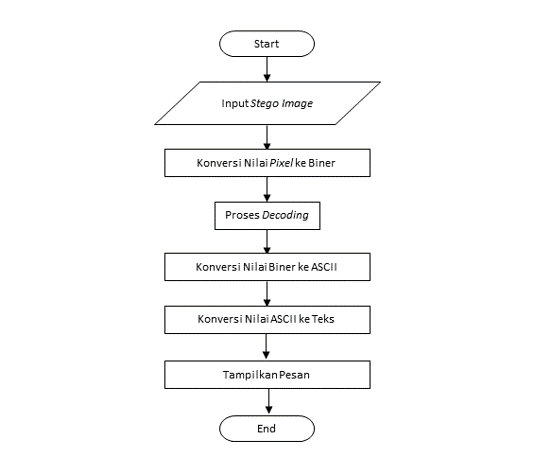
\includegraphics[height=0.6\textheight]{gambar/ekstraksi3}
		\caption{\emph{Flowchart} Ekstraksi Pesan Rahasia}
		\label{flowchart_ekstraksi}
	\end{figure}

	Pada gambar di atas adalah \emph{flowchart} proses ekstraksi pesan dari \emph{Stego Image} yang menghasilkan \emph{Hiddentext} yang terdapat di dalamnya. Prosesnya dimulai dengan
	membaca \emph{file} citra, dan mengubah \emph{pixel} ke dalam nilai biner.
	Kemudian proses ekstraksi (\emph{Decoding}). Setelah diperoleh bit-bit yang tersembunyi pada \emph{Cover Image} maka proses
	berikutnya adalah mengkonversi kembali pesan yang tersembunyi (\emph{Hiddentext}), sehingga pesan dapat ditampilkan kembali.

	\subsection{Desain Antar Muka Program}
	
	Berikut adalah desain antar muka dari program steganografi yang dibangun dengan menggunakan Matlab.
	
	\begin{figure}[H]
		\centering
		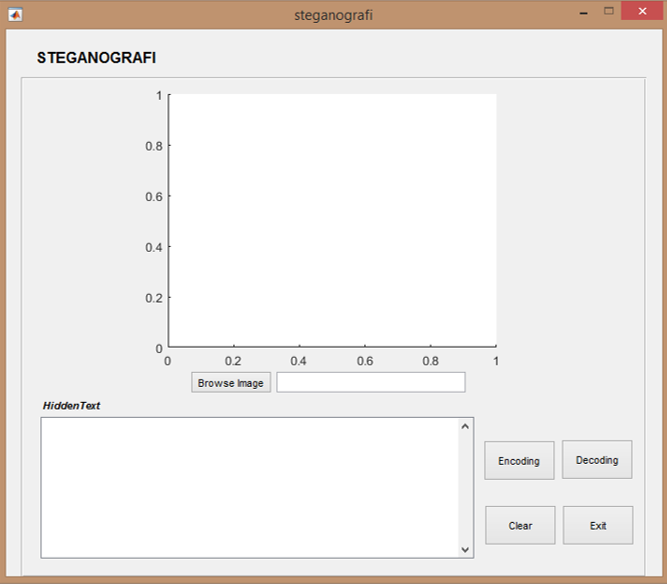
\includegraphics[width=1\textwidth]{gambar/mockup/1}
		\caption{Desain \emph{Form} Steganografi}
		\label{desain_form}
	\end{figure}

	Dari tampilan tersebut, pengambilan gambar yang akan dijadikan sebagai \emph{Cover Image} dilakukan dengan menekan tombol "\emph{Browse Image}" dan gambar akan tampil. 
	
	\begin{figure}[H]
		\centering
		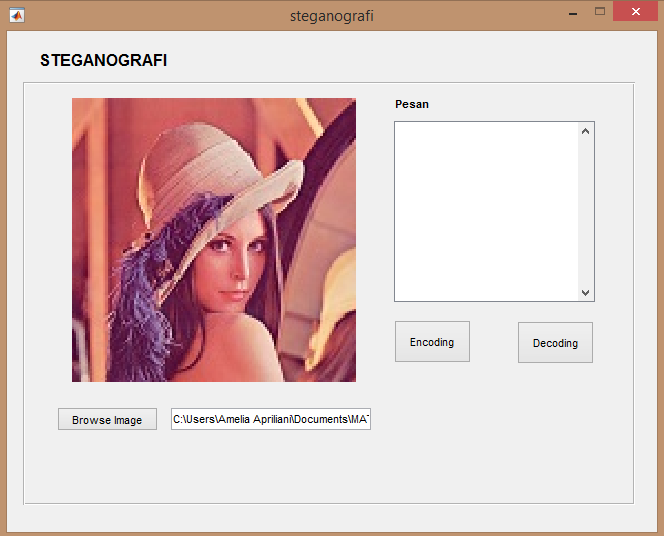
\includegraphics[width=1\textwidth]{gambar/mockup/2}
		\caption{Desain \emph{Form} - \emph{Cover Image}}
		\label{desain_image}
	\end{figure}

	Setelah \emph{Cover Image} tampil maka pesan yang akan disisipkan atau \emph{Hiddentext} dapat dituliskan pada kolom pesan. Dan kemudian klik tombol \emph{Encoding} untuk melakukan proses \emph{Encoding}. Setelah proses \emph{Encoding}, maka akan didapatkan \emph{Stego Image} dan disimpan di folder yang sama.
	
	\begin{figure}[H]
		\centering
		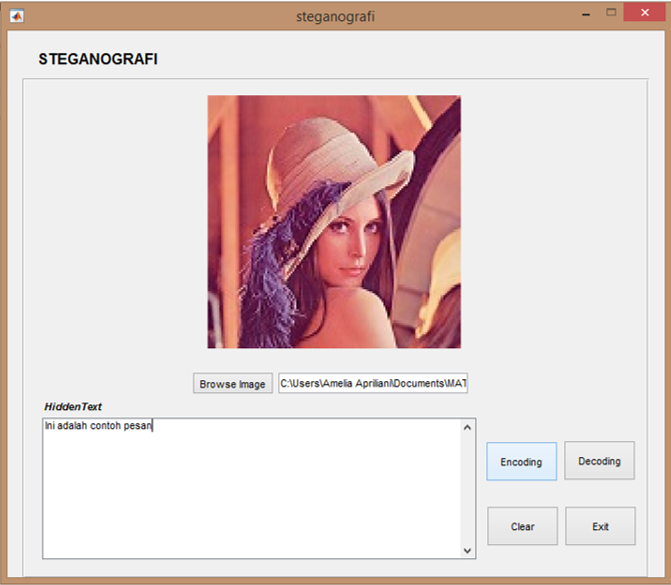
\includegraphics[width=1\textwidth]{gambar/mockup/3}
		\caption{Desain \emph{Form} - Proses \emph{Encoding}}
		\label{desain_encoding}
	\end{figure}

	Jika ingin melakukan proses \emph{Decoding}, maka buka \emph{Stego Image} yang telah disimpan. Kemudian klik tombol \emph{Decoding} dan pesan akan didapatkan.
	
	\begin{figure}[H]
		\centering
		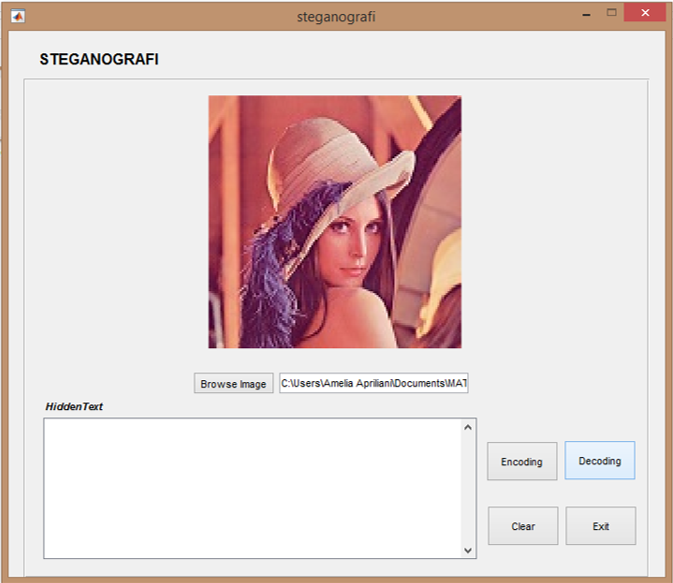
\includegraphics[width=1\textwidth]{gambar/mockup/4}
		\caption{Desain \emph{Form} - Proses \emph{Decoding}}
		\label{desain_decoding}
	\end{figure}

	\begin{figure}[H]
		\centering
		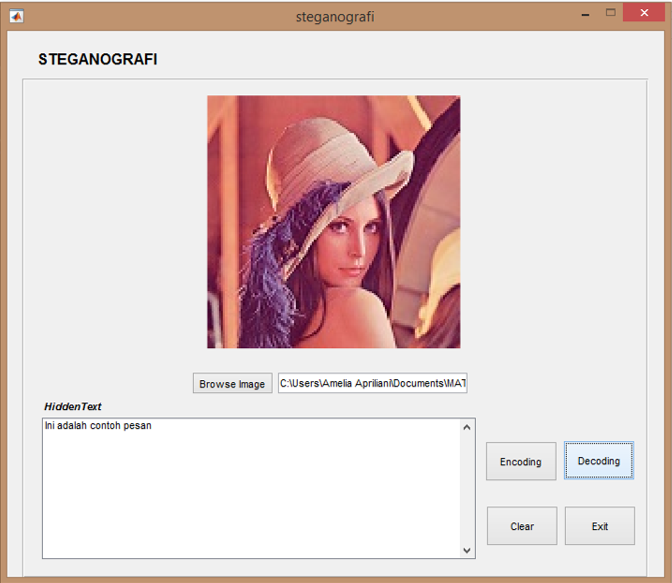
\includegraphics[width=1\textwidth]{gambar/mockup/5}
		\caption{Desain \emph{Form} - Pesan Hasil \emph{Decoding}}
		\label{desain_pesan}
	\end{figure}

\section{Program Steganografi dengan Metode LSB}
	\subsection{\emph{Encoding}}
	\subsection{\emph{Decoding}}
	
\section{Hasil Steganografi}